\chapter{分数视角：从能量模型到 NCSN}\label{ch:score-based}



上一章把扩散模型追溯到它的变分根源，说明了它如何从 VAE 的框架中产生。本章转向另一个同样基本的视角：\emph{能量模型}（EBM）~\citep{ackley1985learning,lecun2006tutorial}。EBM 用一个能量地形来表示分布：在数据上能量低，在别处能量高。采样通常依靠朗之万动力学，它沿着这一能量地形的梯度移动样本，使样本走向高密度区域；这个梯度场称为\emph{分数}，它指向概率更高的方向。

关键的观察是：只要知道分数，就足以完成生成——它能把样本推向更可能的区域，而无需计算那个难以处理的归一化常数。\emph{基于分数}的扩散模型正是建立在这一想法之上。它们不只关注干净数据的分布，而是考虑一族经过高斯噪声扰动的分布，因为这些分布的分数更容易近似。学好这些分数，就得到一族向量场，可以引导噪声样本一步步回到数据，从而把生成变成渐进式的去噪。


\chapterlearning{
  \item 理解基于分数建模的核心思想：分数函数是什么，以及如何把它与朗之万动力学结合起来做生成；
  \item 理解去噪分数匹配如何借助条件化技巧学习单一噪声水平上的分数，以及 Tweedie 公式如何把分数预测与去噪联系起来；
  \item 理解噪声条件分数网络（NCSN）如何把去噪分数匹配推广到多个噪声水平、这样做的益处何在，以及 NCSN 的分数预测与 DDPM 的噪声预测之间有何关系。
}{
已熟悉能量模型的读者可以略过 \Cref{sec:ebm}，直接从 \Cref{subsec:training-sm} 开始。
}



\newpage


\newpage


\section{能量模型}\label{sec:ebm}

对已经熟悉 EBM 的读者，本节是一个简明的回顾，同时也是通往扩散的基于分数视角的桥梁。
\subsection{用能量函数建模概率分布}

设 $\mathbf{x} \in \mathbb{R}^D$ 表示一个数据点。EBM 通过能量函数 $E_{\bm{\phi}}(\mathbf{x})$（由 ${\bm{\phi}}$ 参数化）来定义概率密度，它给更可能的配置分配更低的能量。得到的分布为
\begin{align*}
    p_{{\bm{\phi}}}(\mathbf{x}) := \frac{\exp(-E_{\bm{\phi}}(\mathbf{x}))}{Z_\bphi}, \quad
    Z_\bphi := \int_{\mathbb{R}^D} \exp(-E_{\bm{\phi}}(\mathbf{x})) \diff\mathbf{x},
\end{align*}
其中 $Z_\bphi$ 称为\emph{配分函数}，用来保证归一化：
\[
\int_{\mathbb{R}^D} p_{{\bm{\phi}}}(\mathbf{x})  \diff\mathbf{x} = 1.
\]
\begin{figure}[th!]
    \centering
    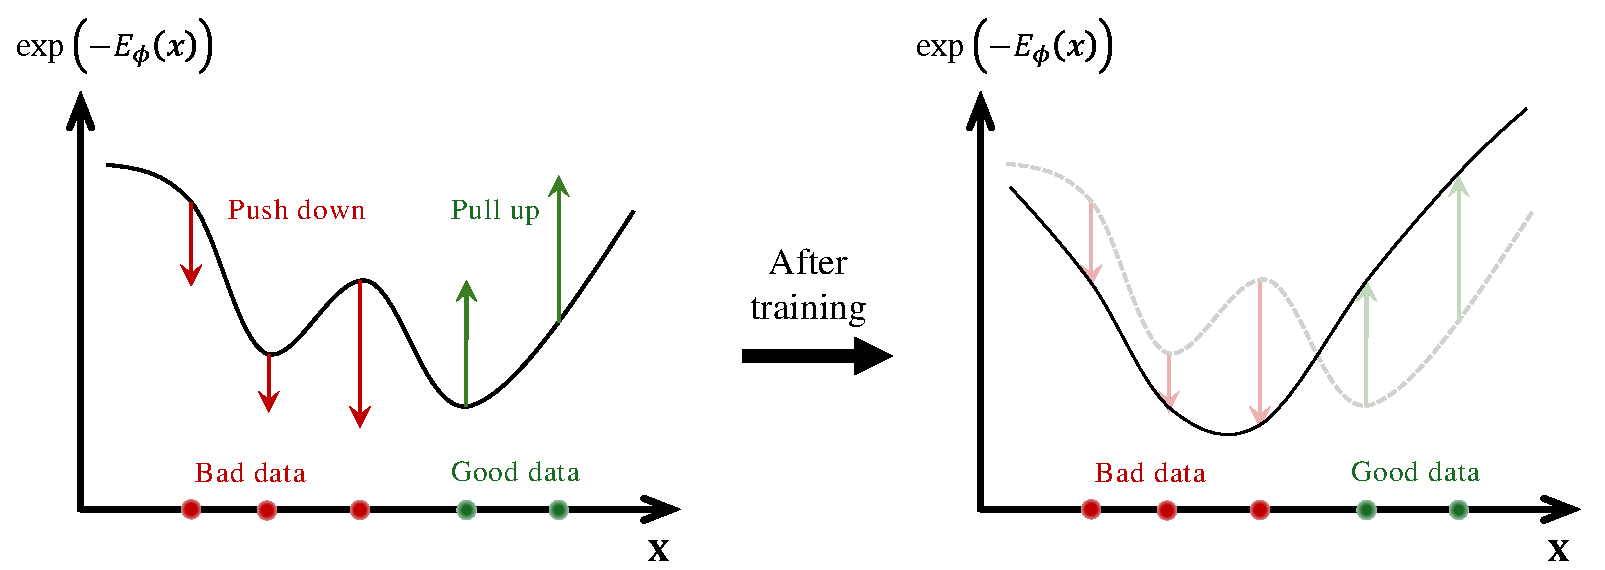
\includegraphics[width=\linewidth]{Images/PartB/ebm-graph.pdf}
    \caption{\textbfs{EBM 训练示意图。} 模型在``坏''数据点处降低密度（抬高能量，红色箭头），在``好''数据点处提高密度（降低能量，绿色箭头）。 \figcredit{由作者创建。}}
        \label{fig:ebm-graph}
\end{figure}

按这一观点，能量较低的点对应较高的概率，就像一个球滚进山谷。配分函数 $Z_{\bphi}$ 保证所有概率之和为一，因此只有能量的\emph{相对}取值才有意义。例如，给所有能量加上同一个常数，分子与分母会乘上同一个因子，分布保持不变。

此外，正因为配分函数 $Z_{\bphi}$ 强制概率总和为一，从数学上可以推出：降低某个区域内的能量会提高该区域的概率，而其补集的概率则相应下降。因此 EBM 服从一种严格的全局权衡：把一个山谷挖得更深，必然使其他山谷变浅，概率质量是在整个空间上重新分配，而不是各自独立地分配给每个区域。


\paragraph{EBM 中最大似然训练的挑战。}
原则上，EBM 可以用最大似然来训练，它自然地平衡了拟合数据与全局正则化（见 \Cref{eq:MLE}）：
\begin{align}
\label{eq:mle-ebm}
\mathcal{L}_{\text{MLE}}(\bphi)
&= \mathbb{E}_{p_{\text{data}}(\rvx)}  \left[ \log \frac{\exp(-E_{\bphi}(\rvx))}{Z_\bphi} \right] \\
&= -  \underbrace{\mathbb{E}_{p_{\text{data}}}[E_{\bphi}(\rvx)]}_{\text{降低数据的能量}}
   -  \underbrace{\log \int \exp(-E_{\bphi}(\rvx))\diff\rvx}_{\text{全局正则化}}, \nonumber
\end{align}
其中 $Z_\bphi = \int \exp(-E_\bphi(\rvx))\diff\rvx$。第一项降低了真实数据的能量，而第二项则通过配分函数实现归一化。

然而在高维情形下，计算 $\log Z_{\bphi}$ 及其梯度是难以处理的，因为它需要在模型分布下求期望。这促使人们改用其他目标：要么去近似这一项，例如对比散度 \citep{hinton2002training}；要么通过\emph{分数匹配}把它完全绕开。

下面我们先在 \Cref{subsec:motivation-score} 中引入分数函数的概念，在 \Cref{subsec:training-ebm} 中把分数匹配作为绕过配分函数的可处理训练目标，最后在 \Cref{subsec:sampling-ebm} 中讨论以分数函数为基础的实用采样方法——朗之万动力学。



\subsection{动机：什么是分数函数？}\label{subsec:motivation-score}

设 $p(\rvx)$ 是定义在 $\mathbb{R}^D$ 上的密度，\emph{分数函数}定义为对数密度的梯度：
\[
\rvs(\rvx) := \nabla_{\rvx} \log p(\rvx), \qquad \rvs \colon \mathbb{R}^D \to \mathbb{R}^D.
\]
直观上，分数构成一个指向概率较高区域的向量场，相当于在局部指示数据最可能出现的位置（见 \Cref{fig:score-function}）。

\begin{figure}[th]
    \centering
    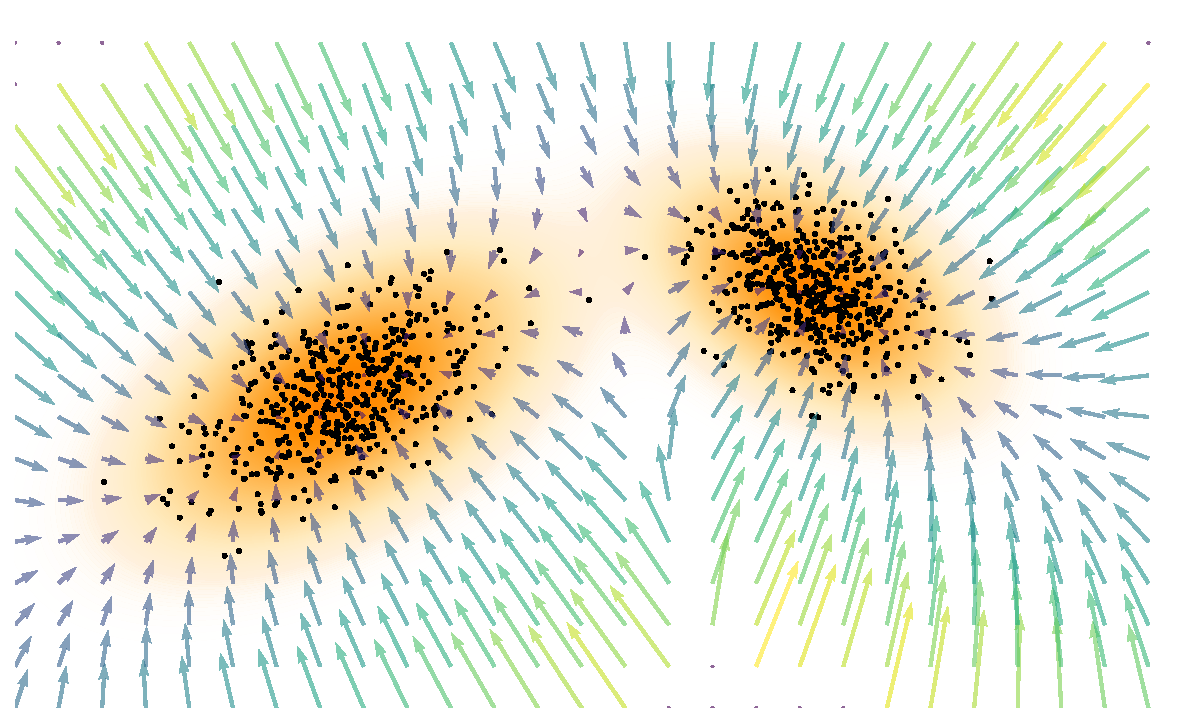
\includegraphics[width=0.95\linewidth]{Images/PartB/score_function_plot.pdf}
    \caption{\textbfs{分数向量场示意图。} 向量场 $\nabla_{\rvx} \log p(\rvx)$ 指示密度增大的方向。 \figcredit{由作者创建。}}
    \label{fig:score-function}
\end{figure}

\paragraph{为什么建模分数而不是密度？}
对分数建模在理论和实践上都有好处：

\subparagraph{1. 不受归一化常数的影响。}\mbox{}\\
     许多分布只以非归一化密度 $\tilde{p}(\rvx)$ 的形式给出，例如 EBM 中的 $\exp(-E_{\bm{\phi}}(\rvx))$：
    \[
    p(\rvx) = \frac{\tilde{p}(\rvx)}{Z},
    \qquad
    Z = \int \tilde{p}(\rvx)\diff\rvx.
    \]
    计算 $Z$ 通常很困难，但分数只依赖于 $\tilde{p}$：
\begin{align}\label{eq:score-compute}
\nabla_{\rvx}\log p(\rvx) = \nabla_{\rvx}\log \tilde{p}(\rvx) - \underbrace{\nabla_{\rvx}\log Z}_{=0} = \nabla_{\rvx}\log \tilde{p}(\rvx), \end{align}
    因为 $Z$ 对 $\rvx$ 而言是常数。这就完全绕开了配分函数。

\subparagraph{2. 完整的表示。}
分数函数完全刻画了底层的分布。由于它是对数密度的梯度，原则上可以把它积分回去，从而恢复密度（至多相差一个常数）：
\[
\log p(\rvx)
= \log p(\rvx_0) + \int_0^1 \rvs(\rvx_0 + t(\rvx - \rvx_0))^\top (\rvx - \rvx_0)  \diff t,
\]
其中 $\rvx_0$ 是参考点，$\log p(\rvx_0)$ 由归一化条件确定。因此，对分数建模与对 $p(\rvx)$ 本身建模具有相同的表达能力，而前者通常更有利于生成建模。


\subsection{通过分数匹配训练 EBM}\label{subsec:training-ebm}
在 EBM 中，密度定义为 $p_{{\bm{\phi}}}(\mathbf{x}) = \tfrac{\exp(-E_{\bm{\phi}}(\mathbf{x}))}{Z_\bphi}$。最大似然训练需要计算 $Z_{\bm{\phi}}$，而这通常难以处理。一个关键的观察是，模型分布 $p_{{\bm{\phi}}}$ 的分数可以化简为 $-\nabla_{\rvx}E_{\bm{\phi}}(\rvx)$，与 $Z_{\bm{\phi}}$ 无关（见 \Cref{eq:score-compute}）。

\emph{分数匹配}~\citep{hyvarinen2005estimation} 正是利用了分数只依赖于能量函数这一事实。它不去拟合归一化后的概率，而是通过让模型分数对齐（未知的）数据分数来训练 EBM：
\begin{align}\label{eq:ebm-sm}
    \mathcal{L}_{\mathrm{SM}}(\bm{\phi})
= \tfrac{1}{2}  \mathbb{E}_{p_{\mathrm{data}}(\mathbf{x})}
\big\| \nabla_{\mathbf{x}} \log p_{\bm{\phi}}(\mathbf{x})
- \nabla_{\mathbf{x}} \log p_{\mathrm{data}}(\mathbf{x}) \big\|_2^2.
\end{align}

虽然数据分数无法直接获取，但通过分部积分可以得到一个只涉及能量及其导数的等价表达式（详见命题~\ref{sm-trace}）：
\[
\mathcal{L}_{\mathrm{SM}}(\bm{\phi}) =
\mathbb{E}_{p_{\mathrm{data}}(\mathbf{x})} \left[
-\Tr \big(\nabla_{\mathbf{x}}^2 E_{\bm{\phi}}(\rvx)\big)
+ \tfrac{1}{2}  \|\nabla_{\mathbf{x}} E_{\bm{\phi}}(\rvx)\|_2^2
\right] + C,
\]
其中 $\nabla_{\mathbf{x}}^2 E_{\bm{\phi}}(\rvx)$ 是 $E_{\bm{\phi}}$ 的黑塞矩阵，$C$ 是不依赖于 $\bm{\phi}$ 的常数。这种写法很有吸引力：它消除了配分函数，也避免了训练期间从模型中采样。它的主要缺点是要求二阶导数：虽然只需黑塞矩阵的迹 $\Tr \big(\nabla_{\mathbf{x}}^2 E_{\bm{\phi}}\big)$ 而非完整的黑塞矩阵，但精确计算这一项通常需要聚合各输入坐标上的二阶导数信息，因此其代价一般随输入维数 $D$ 增长。本章稍后我们会再讨论如何绕开这一限制。




\subsection{用分数函数做朗之万采样}\label{subsec:sampling-ebm}
要从由能量函数 $E_{\bm{\phi}}(\mathbf{x})$ 定义的 EBM 中采样，可以使用\emph{朗之万动力学}。我们先给出离散时间的朗之万更新，再取其连续时间极限，得到一个随机微分方程（SDE）。最后讨论朗之万动力学为何能高效地探索复杂的能量地形，这背后的物理直觉是什么。
\begin{figure}
    \centering
    \includegraphics[width=\linewidth]{Images/PartB/langevin_sampling.png}
    \vspace{-1.5cm}
    \caption{\textbfs{朗之万采样示意图。} 朗之万采样利用分数函数 $\nabla_{\mathbf{x}} \log p_{\bm{\phi}}(\mathbf{x})$，按 \Cref{eq:discrete-langevin-score} 中的更新规则把轨迹引向高密度区域（箭头所示）。 \figcredit{由作者创建。}}
        \label{fig:langevin}
\end{figure}


\paragraph{离散时间朗之万动力学。}
离散时间的朗之万更新为
\begin{align}\label{eq:discrete-langevin}
    \mathbf{x}_{n+1} = \mathbf{x}_n - \eta \nabla_{\mathbf{x}} E_{\bm{\phi}}(\mathbf{x}_n) +  \sqrt{2 \eta} \bm{\epsilon}_n, \quad n=0,1,2,\ldots,
\end{align}
其中 $\mathbf{x}_0$ 从某个分布（通常是高斯分布）中初始化，$\eta > 0$ 是步长，$\bm{\epsilon}_n \sim \mathcal{N}(\mathbf{0}, \mathbf{I})$ 是高斯噪声。噪声带来的随机性使探索能够越过局部极小值。

由于分数函数可以写成
\[
\nabla_{\mathbf{x}} \log p_{\bm{\phi}}(\mathbf{x}) = -\nabla_{\mathbf{x}} E_{\bm{\phi}}(\rvx),
\]
更新也可以等价地写为
\begin{align}\label{eq:discrete-langevin-score}
    \mathbf{x}_{n+1} = \mathbf{x}_n + \eta \nabla_{\mathbf{x}} \log p_{\bm{\phi}}(\mathbf{x}_n) + \sqrt{2 \eta}\bm{\epsilon}_n,
\end{align}
其中分数函数引导样本走向高密度区域。这一形式是扩散模型的核心，后文会详细介绍。

\paragraph{连续时间朗之万动力学。}
当步长 $\eta$ 趋于零时，离散朗之万更新自然收敛到由\emph{朗之万随机微分方程（SDE）}\footnote{ 描述的连续时间过程。借助 $\sqrt{2}$ 这一因子，朗之万动力学使 $p_{\bm\phi}$ 随时间保持不变。也就是说，$p_{\bm\phi}$ 是平稳分布：若 $\rvx(0)\sim p_{\bm\phi}$，则对任意 $t\ge 0$ 都有 $\rvx(t)\sim p_{\bm\phi}$。等价地，$p_{\bm\phi}$ 是福克尔-普朗克方程的平稳解（见 \Cref{app:continuity}）：
\[
\partial_t \rho = -\nabla \cdot(\rho  \nabla\log p_{\bm\phi}) + \tfrac{\sigma^2}{2}\Delta \rho.
\]
代入 $\rho=p_{\bm\phi}$ 可得 $(\tfrac{\sigma^2}{2}-1)\Delta p_{\bm\phi}=0$，它仅在 $\sigma=\sqrt{2}$ 时成立。
}：
\begin{align}\label{eq:continuous-langevin}
 \diff \mathbf{x}(t) = \nabla_{\mathbf{x}} \log p_{\bm{\phi}}(\mathbf{x}(t)) \diff t + \sqrt{2} \diff \mathbf{w}(t),
\end{align}
其中 $\mathbf{w}(t)$ 表示标准布朗运动（又称维纳过程\footnote{布朗增量满足
$\mathbf{w}(t+\eta)-\mathbf{w}(t)\sim \mathcal{N}(\mathbf{0},  \eta  \mathbf{I})$。
因此 Euler--Maruyama 格式使用的噪声为 $\sqrt{2}  [\mathbf{w}(t+\eta)-\mathbf{w}(t)]
= \sqrt{2\eta}  \bm{\epsilon}_n$，其中 $\bm{\epsilon}_n \sim \mathcal{N}(\mathbf{0},\mathbf{I})$，这就解释了 $\sqrt{\eta}$ 这一因子，也是平方根缩放的来源。关于布朗运动与 SDE 的详细介绍，见 \Cref{app:de}。}）。需要理解的是，\Cref{eq:discrete-langevin} 中的离散更新规则正是该连续 SDE 的 Euler--Maruyama 离散化。



在标准的正则性假设下（例如 $p_{\bm{\phi}}\propto e^{-E_{\bm{\phi}}}$，且 $E_{\bm{\phi}}$ 有限、足够光滑），$\mathbf{x}(t)$ 的分布会（以指数速度）收敛到 $p_{\bm{\phi}}$（当 $t\to\infty$）；因此只需模拟（求解）SDE \Cref{eq:continuous-langevin} 即可完成采样。

\paragraph{为什么要用朗之万采样？}
理解朗之万采样的一种自然方式是从物理视角出发：能量函数 $ E_{\bm{\phi}}(\mathbf{x}) $ 定义了一个支配粒子行为的势能地形。按牛顿力学，粒子在该能量所导出的力场中的运动由常微分方程（ODE）描述：
\[
\diff \mathbf{x}(t) = -\nabla_{\mathbf{x}} E_{\bm{\phi}}\big(\mathbf{x}(t)\big)  \diff t,
\]
它确定性地驱动粒子向能量函数的局部极小值下降。然而这种确定性动力学可能被困在局部极小值中，从而妨碍对整个数据分布的探索。

为克服这一限制，朗之万动力学引入随机扰动，由此得到 SDE
\[
\diff \mathbf{x}(t) = -\nabla_{\mathbf{x}} E_{\bm{\phi}}\big(\mathbf{x}(t)\big)  \diff t + \underbrace{\sqrt{2 } \diff \rvw(t)}_{\text{注入的噪声}},
\]
其中 $\rvw(t)$ 是标准布朗运动。

噪声项使粒子能够越过能量壁垒、逃离局部极小值，使轨迹成为一个随机过程，其平稳分布收敛到玻尔兹曼分布
\[
p_{\bm{\phi}}(\mathbf{x}) \propto e^{-E_{\bm{\phi}}(\mathbf{x})}.
\]

从这个角度看，EBM 可以视为在学习一个把样本推向高概率区域的力场。朗之万采样对 EBM 尤其有用，因为它提供了一种从模型分布 $p_{\bm{\phi}}(\mathbf{x})$ 生成样本的实用方法，而无需显式计算配分函数：反复应用朗之万更新，即可得到近似目标分布的样本。


\paragraph{朗之万采样的固有困难。}
朗之万动力学是一种广泛使用的基于 MCMC 的采样器，但在高维空间中面临严重局限。它的效率对步长 $\eta$、噪声尺度，以及精确逼近目标分布所需的迭代次数都非常敏感。

这种低效率的根源是混合时间（mixing time）过长：对于含许多孤立模态的复杂数据分布，朗之万采样常常需要极长时间才能在高概率区域之间迁移，而且随着维数升高这一问题更加严重，导致收敛过慢。

可以把采样想象为探索一片广阔而崎岖的地形，其中散落着许多彼此遥远的山谷，每个山谷对应数据的一个模态。朗之万动力学依赖局部的随机更新，难以有效地跨越这些山谷，因此往往无法覆盖分布的全部多样性。

这种低效也提示我们：需要更结构化、更有引导性的采样方法，才能比纯粹的随机探索更有效地穿行于复杂的数据流形。

\newpage

\section{从能量模型到基于分数的生成模型}
EBM 表明，生成只取决于分数——它指向概率更高的区域，而不需要完全归一化的密度。虽然分数匹配绕开了配分函数，但经由能量来训练仍然需要昂贵的二阶导数。关键的想法是：既然朗之万采样只需要分数，我们就可以直接用神经网络来学习分数本身。这种从建模能量到建模分数的转变，构成了基于分数的生成模型的基础。

\begin{figure}[ht!]
    \centering
    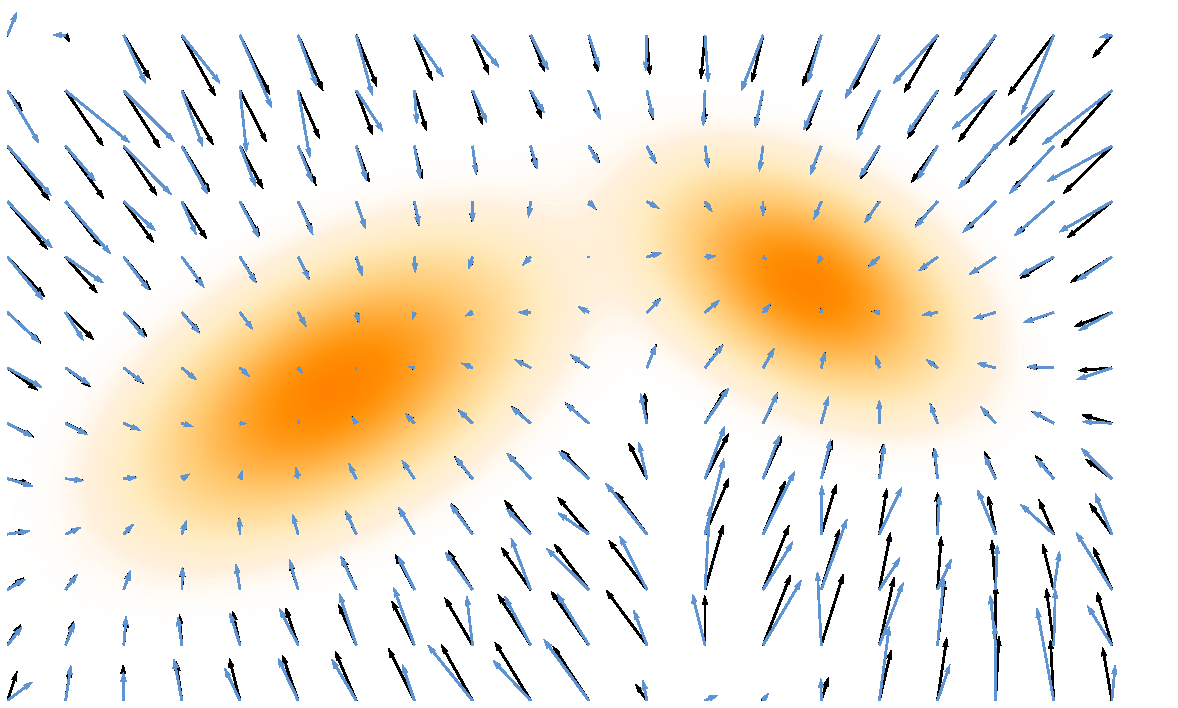
\includegraphics[width=0.9\linewidth]{Images/PartB/score_function_approximation.pdf}
    \caption{\textbfs{分数匹配示意图。} 神经网络分数 ${\color{customblue}\rvs_{\bm{\phi}}(\rvx)}$ 通过 MSE 损失训练，以匹配真实分数 $\rvs(\rvx)$，二者都用向量场表示。 \figcredit{由作者创建。}}
        \label{fig:sm-illustration}
\end{figure}

\subsection{使用分数匹配进行训练}\label{subsec:training-sm}
\paragraph{分数匹配。}
分数函数 $\rvs(\rvx) = \nabla_{\rvx} \log p_{\mathrm{data}}(\rvx)$ 只通过 $p_{\mathrm{data}}$ 的样本给出，我们直接用神经网络参数化的向量场 $\rvs_{\bm{\phi}}(\rvx)$ 去近似它（见 \Cref{fig:sm-illustration}）：
\[
\rvs_{\bm{\phi}}(\rvx) \approx \rvs(\rvx).
\]
\emph{分数匹配}通过最小化真实分数与估计分数之间的均方误差（MSE）来拟合这一向量场：
\begin{mdframed}
\begin{align}\label{eq:sm}
    \mathcal{L}_{\mathrm{SM}}(\bm{\phi})
    := \frac{1}{2}  \mathbb{E}_{\rvx \sim p_{\mathrm{data}}}
    \Big[\| \rvs_{\bm{\phi}}(\rvx) - \rvs(\rvx)\|_2^2\Big].
\end{align}
\end{mdframed}

\paragraph{可处理的分数匹配。}
乍看之下这个目标似乎无从下手：作为回归目标的真实分数
$\rvs(\rvx)$ 是未知的。所幸 \citet{hyvarinen2005estimation} 指出，通过分部积分可以得到一个等价的、只依赖于模型 $\rvs_{\bm{\phi}}$ 和数据样本的目标，无需拿到真实分数。下面用命题给出这一关键结果：
\proppp{Hyvärinen 的 SM 易处理形式}{sm-trace}
        {
        有下面的等式成立：
        \begin{align*}
            \mathcal{L}_{\text{SM}}(\bm{\phi}) = \widetilde{\mathcal{L}}_{\text{SM}}(\bm{\phi}) + C.
        \end{align*}
        其中
        \begin{align}\label{eq:sm-alternative}
            \widetilde{\mathcal{L}}_{\text{SM}}(\bm{\phi})
            := \mathbb{E}_{\rvx \sim p_{\text{data}}(\rvx)} \left[
            \Tr\left(\nabla_{\rvx}\rvs_{\bm{\phi}}(\rvx)\right)
            + \frac{1}{2} \norm{\rvs_{\bm{\phi}}(\rvx)}_2^2
            \right].
        \end{align}
        且 $C$ 是不依赖于 $\bm{\phi}$ 的常数。其最小解为 $\rvs^*(\cdot) = \nabla_{\rvx} \log p(\cdot)$。
        }
        {证明把 MSE 展开为 $ \mathcal{L}_{\text{SM}} $ 的形式，再应用分部积分。见 \Cref{app-sec:sm-trace}。
        }

利用等价目标 \Cref{eq:sm-alternative}，我们就可以只从观测样本 $p_{\mathrm{data}}$ 训练分数模型 $\rvs_{\bm{\phi}}(\rvx)$，不再需要真实分数函数。

\paragraph{\Cref{eq:sm-alternative} 的直觉。}
替代的分数匹配目标 $\widetilde{\mathcal{L}}_{\text{SM}}(\bm\phi)$
可以从它的两项来理解。
范数项 $\tfrac12\|\rvs_{\bm\phi}(\rvx)\|^2$ 惩罚过大的分数值，
在 $p_{\mathrm{data}}$ 较大的区域尤其如此。
散度项 $\Tr(\nabla_{\rvx} \rvs_{\bm\phi}(\rvx))$ 在损失中以正号出现，因此最小化目标也会促使局部收缩。
两项合起来，就给出了总体最优的分数场
$\rvs^*(\rvx)=\nabla_{\rvx}\log p_{\mathrm{data}}(\rvx)$。
下面更详细地解释其中的几何直觉。

\subparagraph{幅值项的作用。}
由于 $\widetilde{\mathcal{L}}_{\mathrm{SM}}(\bm\phi)$ 中的期望是对
$p_{\mathrm{data}}$ 取的，$p_{\mathrm{data}}(\rvx)$ 较大的区域（数据密度高）
对损失的贡献更大。因此幅值项
$\tfrac12\|\rvs_{\bm\phi}(\rvx)\|^2$ 会压制这些区域中过大的分数值。不过这一项本身并不意味着在每个高密度点上都有 $\rvs_{\bm\phi}(\rvx)=\mathbf{0}$；在总体最优解处，
\[
\rvs^*(\rvx)=\nabla_{\rvx}\log p_{\mathrm{data}}(\rvx),
\]
它只在（对数密度的）驻点处才为零。

\subparagraph{场为（近似）梯度时的凹性。}
散度项 $\Tr(\nabla_{\rvx} \rvs_{\bm\phi}(\rvx))$ 在损失中以正号出现，因此最小化目标倾向于在数据分布集中的区域会出现负的散度。散度为负意味着局部净收缩，不过它本身并不保证驻点就是汇点。
为把这一点说清，假设
$\rvs_{\bm\phi}=\nabla_{\rvx}u$，其中 $u:\R^D\to\R$ 是标量函数，此时模型正是在匹配对数密度。于是 $\nabla_{\rvx}\rvs_{\bm\phi}=\nabla_{\rvx}^2 u$（黑塞矩阵），而
$\nabla \cdot \rvs_{\bm\phi}(\rvx)=\Tr(\nabla_{\rvx}^2 u(\rvx))$（散度）。

在驻点 $\rvx_\star$，其中 $\rvs_{\bm\phi}(\rvx_\star)=\nabla_{\rvx}u(\rvx_\star)=\mathbf{0}$，
二阶泰勒展开式给出
\[
u(\rvx)
= u(\rvx_\star)
+ \tfrac12(\rvx-\rvx_\star)^\top \nabla_{\rvx}^2 u(\rvx_\star)(\rvx-\rvx_\star)
+ o(\|\rvx-\rvx_\star\|^2).
\]
如果黑塞矩阵 $\nabla_{\rvx}^2 u(\rvx_\star)$ 负定，则 $u$ 在
$\rvx_\star$ 处局部凹，对数密度在该点取得严格的局部极大值\footnote{ 注意，严格的凹性（从而是对数密度的严格局部极大值）要求整个黑塞矩阵
$\nabla_{\rvx}^2 u$ 负定，而不仅仅是迹为负。
迹为负只能保证特征值之和为负，某些特征值仍可能为正，从而得到鞍点而非极大值。
}。
由于黑塞矩阵的所有特征值均为负，其迹也必为负：
$\Tr(\nabla_{\rvx}^2 u(\rvx_\star))<0$。
因此在这种情况下，该驻点在分数场下具有局部吸引性：
微小的扰动都会被拉向 $\rvx_\star$。

\subsection{用朗之万动力学采样}
通过最小化 \Cref{eq:sm-alternative} 训练完成后，就可以用分数模型 $\rvs_{\bm{\phi}^\times}(\rvx)$ 替换朗之万动力学中的预言（oracle）分数来做采样：
\begin{align}\label{eq:score-langevin-emp}
    \mathbf{x}_{n+1} = \mathbf{x}_n + \eta   \rvs_{\bm{\phi}^\times}(\rvx_n) + \sqrt{2\eta}    \bm{\epsilon}_n, \quad \bm{\epsilon}_n \sim \mathcal{N}(\bm{0}, \bm{I}),
\end{align}
其中 $n=0,1,2,\dots$，初始点取 $\rvx_0$。与 EBM 的情形（\Cref{eq:continuous-langevin}）一样，这个递推正是连续时间朗之万 SDE 的 Euler--Maruyama 离散化：
\begin{align*}
    \diff \rvx(t) = \rvs_{\bm{\phi}^\times}(\rvx(t)) \diff t + \sqrt{2} \diff \mathbf{w}(t),
\end{align*}
初值为 $\rvx(0)$。因此在小步长极限下，离散格式与连续格式是一致的。实践中既可以运行离散采样器，也可以直接模拟 SDE。



\subsection{引言：基于分数的生成模型}

在本章余下部分，我们考察分数函数在现代扩散模型中的基础作用。分数函数最初是为了高效训练 EBM 而引入的，如今已成为新一代生成模型的核心构件。在此之上，我们讨论分数函数如何同时指导 \emph{基于分数的扩散模型}的理论构建与实际实现，为借助随机过程生成数据提供一个有原则的框架。



\newpage


\section{去噪分数匹配}\label{sec:dsm}

\subsection{动机}
虽然替代目标 \Cref{eq:sm-alternative}
\begin{align*}
    \widetilde{\mathcal{L}}_{\text{SM}}(\bm{\phi}) = \mathbb{E}_{\rvx \sim p_{\mathrm{data}}} \left[\mathrm{Tr}\big(\nabla_{\rvx}\rvs_{\bm{\phi}}(\rvx)\big) + \frac{1}{2} \|\rvs_{\bm{\phi}}(\rvx)\|_2^2 \right]
\end{align*}
虽然更容易处理，但仍需计算雅可比矩阵的迹 $\mathrm{Tr}(\nabla_{\rvx}\rvs_{\bm{\phi}}(\rvx))$。虽然不必显式构造完整的雅可比矩阵，但精确计算这一项通常需要聚合各输入坐标上的导数信息，因此代价随输入维数 $D$ 增长；在高维情形下会变得相当昂贵。为此，切片分数匹配~\citep{song2020sliced} 用一个基于随机投影的随机估计替换迹项。下面简述其思路。

\paragraph{切片分数匹配与 Hutchinson 估计器。} 切片分数匹配的做法是：沿随机的“切片”方向求方向导数，再对这些导数取平均，以此替代分数匹配中的迹项。设 $\rvu\in\R^D$ 为\emph{各向同性}随机向量（例如 Rademacher 向量或标准高斯向量），满足 $\E[\rvu]=0$ 与 $\E[\rvu\rvu^\top]=\mathbf I$。由 Hutchinson 恒等式
\[
\Tr(\rmA)=\E_{\rvu}[\rvu^\top \rmA \rvu],\quad\text{以及}\quad\E_{\rvu}[(\rvu^\top\rvs_{\bphi}(\rvx))^2]=\|\rvs_{\bphi}(\rvx)\|_2^2,
\]
即可把目标写成精确的等价形式
\[
\widetilde{\mathcal{L}}_{\mathrm{SM}}(\bphi)
=\E_{\rvx,\rvu} \Big[\rvu^\top\big(\nabla_{\rvx}\rvs_{\bphi}(\rvx)\big)\rvu+\tfrac12(\rvu^\top\rvs_{\bphi}(\rvx))^2\Big].
\]
借助自动微分，这一目标可以用雅可比向量积（JVP）或向量雅可比积（VJP）高效计算，而不必显式构造庞大的雅可比矩阵或黑塞矩阵。对 $K$ 个随机探测方向取平均，得到无偏估计，方差为 $\mathcal{O}(1/K)$；其中的方向项 $\rvu^\top(\nabla_{\rvx}\rvs_{\bphi})\rvu$ 同样可以用 JVP/VJP 例程高效求出，无需显式写出雅可比矩阵。直观地说，这种做法只沿随机方向考察模型的行为：把分数投影到随机方向上，并将它推向数据密度更高的区域，于是数据点在期望意义下成为稳定点。

\paragraph{从切片分数匹配到去噪分数匹配。} 切片分数匹配绕开了雅可比矩阵，但仍依赖原始数据分布，因而相当脆弱：对于落在低维流形上的图像数据，分数 $\nabla_{\rvx}\log p_{\mathrm{data}}(\rvx)$ 可能没有定义，也可能数值不稳；而且该方法只在观测点上约束向量场，对这些点邻域的控制很弱，还要额外承担随机探测方向带来的方差和反复计算 JVP/VJP 的开销。

一个更稳健、也是本章重点讨论的替代方案，是\emph{去噪分数匹配}（DSM）~\citep{vincent2011connection}。它既有清晰的理论依据，又能扩展到大规模问题。

\subsection{训练}
让我们重新审视 \Cref{eq:sm} 中的分数匹配损失：
\begin{align*}
     \mathcal{L}_{\text{SM}}(\bm{\phi}) =  \frac{1}{2} \mathbb{E}_{\rvx \sim p_{\text{data}}(\rvx)} \left[ \norm{\rvs_{\bm{\phi}}(\rvx) - \nabla_{\rvx} \log p_{\text{data}}(\rvx)}_2^2 \right],
\end{align*}
麻烦就出在 $\nabla_{\rvx} \log p_{\text{data}}(\rvx)$ 这一难以计算的项上。

\paragraph{\citet{vincent2011connection} 给出的条件化方案。}
为绕开 $\nabla_{\rvx} \log p_{\text{data}}(\rvx)$ 难以计算这一障碍，\citet{vincent2011connection} 提出：先给数据 $\rvx \sim p_{\text{data}}$ 注入噪声，所用的已知条件分布为 $p_{\sigma}(\tilde{\rvx}|\rvx)$，尺度参数为 $\sigma$；再训练神经网络 $\rvs_{\bm{\phi}}(\tilde{\rvx}, \sigma)$ 去逼近扰动后边缘分布的分数
\[
p_\sigma(\tilde{\rvx}) = \int p_{\sigma}(\tilde{\rvx}|\rvx) p_{\text{data}}(\rvx) \diff \rvx,
\]
即最小化如下损失
\begin{align}\label{eq:sm-noise-loss}
\mathcal{L}_{\text{SM}}(\bm{\phi}; \sigma) := \frac{1}{2} \mathbb{E}_{\tilde{\rvx} \sim p_\sigma} \left[ \norm{\rvs_{\bm{\phi}}(\tilde{\rvx}, \sigma) - \nabla_{\tilde{\rvx}} \log p_\sigma(\tilde{\rvx})}_2^2 \right].
\end{align}

尽管 $\nabla_{\tilde{\rvx}} \log p_\sigma(\tilde{\rvx})$ 一般难以计算，\citet{vincent2011connection} 证明：以 $\rvx \sim p_{\text{data}}$ 为条件，可以得到一个等价且易于计算的目标，即\emph{去噪分数匹配}（DSM）损失
\begin{mdframed}
\begin{align}\label{eq:dsm-loss}
\mathcal{L}_{\text{DSM}}(\bm{\phi}; \sigma) := \frac{1}{2} \mathbb{E}_{\rvx \sim p_{\text{data}}, \tilde{\rvx} \sim p_{\sigma}(\cdot|\rvx)} \left[ \norm{\rvs_{\bm{\phi}}(\tilde{\rvx}, \sigma) - \nabla_{\tilde{\rvx}} \log p_{\sigma}(\tilde{\rvx}|\rvx)}_2^2 \right].
\end{align}
\end{mdframed}

\Cref{eq:dsm-loss} 的最优解 $\rvs^*$ 满足
\[
\rvs^*(\tilde{\rvx}, \sigma) = \nabla_{\tilde{\rvx}} \log p_\sigma(\tilde{\rvx}),
\]
它同时也是 \Cref{eq:sm-noise-loss} 的最优解。

以方差为 $\sigma^2$ 的高斯噪声为例，此时
\[
p_{\sigma}(\tilde{\rvx}|\rvx) = \mathcal{N}(\tilde{\rvx}; \rvx, \sigma^2 \mathbf{I}),
\]
梯度 $\nabla_{\tilde{\rvx}} \log p_{\sigma}(\tilde{\rvx}|\rvx)$ 有闭式表达（见 \Cref{eq:gaussian-dsm}），于是回归目标可以直接写出，计算上也完全可行。

此外，当 $\sigma \approx 0$ 时 $p_\sigma(\tilde{\rvx}) \approx p_{\text{data}}(\rvx)$，从而
\[
\rvs^*(\tilde{\rvx}, \sigma) = \nabla_{\tilde{\rvx}} \log p_\sigma(\tilde{\rvx}) \approx \nabla_{\rvx} \log p_{\text{data}}(\rvx),
\]
这说明学到的分数逼近原始数据的分数，因此可以用于生成。

下面这个定理把 $\mathcal{L}_{\text{SM}}$ 与 $\mathcal{L}_{\text{DSM}}$ 在梯度层面的等价性正式表述出来。
\thmp{$\mathcal{L}_{\text{SM}}$ 与 $\mathcal{L}_{\text{DSM}}$ 的等价性}{sm-dsm}{
对任意固定的噪声尺度 $\sigma > 0$，都有
\begin{align}\label{eq:score-matching}
    \mathcal{L}_{\text{SM}}(\bm{\phi}; \sigma) = \mathcal{L}_{\text{DSM}}(\bm{\phi}; \sigma) + C,
\end{align}
其中 $C$ 是与参数 $\bm{\phi}$ 无关的常数。此外，两个损失的最优解 $\rvs^*(\cdot, \sigma)$ 都满足
\[
    \rvs^*(\tilde{\rvx}, \sigma) = \nabla_{\tilde{\rvx}} \log p_\sigma(\tilde{\rvx}), \quad \text{对几乎所有的 } \tilde{\rvx}.
\]
}{等价性可由直接计算得到：把 $\mathcal{L}_{\text{SM}}$ 与 $\mathcal{L}_{\text{DSM}}$ 中的均方误差展开，所有与 $\bm{\phi}$ 相关的项都会相消，只剩下一个与 $\bm{\phi}$ 无关的常数差。\\
最优解的推导沿用命题~\ref{dsm-minimizer} 中相同的论证，详细推导见 \Cref{app-sec:sm-dsm}。
}

这个定理与 DDPM 中的定理~\ref{thm:equiv-marginal-kl} 一样，揭示了一条关键的共通原则：
\msg{洞见}{条件化技巧}{条件化技巧同样出现在 DDPM 中扩散模型的变分视角里（见定理~\ref{thm:equiv-marginal-kl}）：以数据点 $\rvx$ 为条件，就把一个难以计算的损失变成了可以蒙特卡洛估计的可处理损失。基于流的视角中也有类似思路（例如流匹配~\citep{lipman2022flow}），我们将在 \Cref{sec:flow-matching-framework} 中看到。}


\begin{figure}
    \centering
    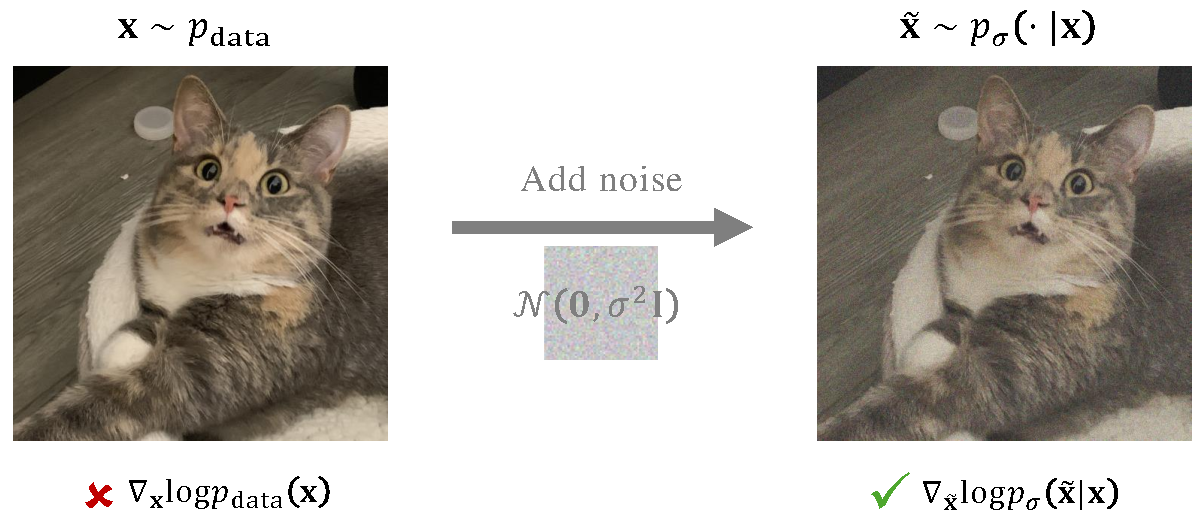
\includegraphics[width=0.8\linewidth]{Images/PartB/dsm-graph.pdf}
    \caption{\textbfs{用条件化技巧说明 DSM。} 用小幅加性高斯噪声 $\mathcal{N}(\mathbf{0}, \sigma^2 \rmI)$ 扰动数据分布 $p_{\mathrm{data}}$，所得的条件分布 $p_{\sigma}(\tilde{\rvx}|\rvx) = \mathcal{N}(\tilde{\rvx}; \rvx, \sigma^2 \rmI)$ 具有闭式的分数函数。
\figcredit{由作者创建。}}
    \label{fig:dsm-graph}
\end{figure}


\paragraph{特殊情形：加性高斯噪声。} 现在考虑最常见的情形：给每个数据点 $\rvx \sim p_{\text{data}}$ 加上方差为 $\sigma^2$ 的高斯噪声 $\mathcal{N}(\mathbf{0}, \sigma^2 \rmI)$，即
\[
\tilde{\rvx} = \rvx + \sigma \bm{\epsilon}, \quad \bm{\epsilon} \sim \mathcal{N}(\mathbf{0}, \rmI),
\]
于是受扰数据 $\tilde{\rvx}$ 服从
\[
p_{\sigma}(\tilde{\rvx}|\rvx) = \mathcal{N}(\tilde{\rvx}; \rvx, \sigma^2 \rmI).
\]
此时条件分数可以解析地写出
\[
\nabla_{\tilde{\rvx}} \log p_{\sigma}(\tilde{\rvx}|\rvx) = \frac{\rvx - \tilde{\rvx}}{\sigma^2}.
\]
于是 DSM 损失简化为：
\begin{mdframed}
\begin{align}\label{eq:gaussian-dsm}
\begin{aligned}
    \mathcal{L}_{\text{DSM}}(\bm{\phi}; \sigma) &= \frac{1}{2} \mathbb{E}_{\rvx, \tilde{\rvx}|\rvx} \left[ \norm{\rvs_{\bm{\phi}}(\tilde{\rvx}, \sigma) - \frac{\rvx - \tilde{\rvx}}{\sigma^2}}_2^2 \right] \\
    &= \frac{1}{2} \mathbb{E}_{\rvx, \bm{\epsilon}} \left[ \norm{\rvs_{\bm{\phi}}(\rvx + \sigma \bm{\epsilon}, \sigma) + \frac{\bm{\epsilon}}{\sigma}}_2^2 \right],
\end{aligned}
\end{align}
\end{mdframed}
其中 $\bm{\epsilon} \sim \mathcal{N}(\mathbf{0}, \rmI)$。这个目标正是（基于分数的）扩散模型的核心。在固定噪声水平 $\sigma>0$ 下，DSM 学的是高斯平滑后分布的分数
\[
p_\sigma
=
p_{\mathrm{data}} * \mathcal{N}(\bm{0},\sigma^2\rmI),
\]
而不是 $p_{\mathrm{data}}$ 本身的分数。$\sigma$ 较小时扰动轻微，$p_\sigma$ 仍紧密保留数据分布的局部结构，因此它的分数能为带噪样本指回可能出现数据的区域，给出有用的移动方向。$\sigma$ 变大时，高斯平滑会逐步抹去细节、把邻近的模态并在一起，相应的分数主要刻画更粗糙、更全局的结构。这一行为恰恰是有用的：\Cref{sec:SMLD} 中的多噪声构造正是有意组合多个噪声水平，用大噪声做粗略探索，用小噪声做精细修正。


为更清楚地看出这一目标为何天然对应“去噪”过程，我们展开 \Cref{subsec:why-dsm-denoising-tweedie,subsec:why-dsm-denoising-sure} 中的讨论。


\subsection{采样}
一旦在噪声水平 $\sigma$ 上训练好分数模型 $\rvs_{\bm{\phi}^\times}(\tilde{\rvx}, \sigma)$，就可以用学到的模型替换真实分数，通过朗之万动力学生成样本。更新规则为：
\begin{align}\label{eq:score-langevin-emp-dsm}
   \tilde{\rvx}_{n+1} = \tilde{\rvx}_n + \eta \underbrace{\rvs_{\bm{\phi}^\times}(\tilde{\rvx}_n, \sigma)}_{\approx \nabla_{\tilde{\rvx}} \log p_\sigma(\tilde{\rvx}_n)} + \sqrt{2\eta}    \bm{\epsilon}_n, \quad \bm{\epsilon}_n \sim \mathcal{N}(\mathbf{0}, \rmI),
\end{align}
其中 $n = 0, 1, 2, \dots$，迭代从初值 $\tilde{\rvx}_0$ 出发。若 $\sigma$ 足够小，则经过充分多轮迭代后，$\tilde{\rvx}_n$ 可近似为 $p_{\text{data}}$ 的样本。


\paragraph{噪声注入的好处。}
此外还值得指出，与 \Cref{eq:sm} 中的原始分数匹配相比，注入高斯噪声形成 $p_\sigma$（例如 \Cref{eq:gaussian-dsm}）带来两个关键优势~\citep{song2019generative}：
\begin{itemize}
  \item \textbfs{梯度处处有定义。} 噪声把数据推离其低维流形，使 $p_\sigma$ 在 $\mathbb{R}^D$ 上具有满支撑。于是分数函数 $\nabla_{\tilde{\rvx}} \log p_\sigma(\tilde{\rvx})$ 处处有明确定义。
  \item \textbfs{覆盖更充分。} 噪声抹平了模态之间的稀疏区域，既提升了训练信号的质量，也让朗之万动力学能更有效地穿过低密度区域。
\end{itemize}


\subsection{为什么 DSM 是去噪：Tweedie 公式}\label{subsec:why-dsm-denoising-tweedie}

我们从\emph{Tweedie 公式}~\citep{efron2011tweedie} 讲起，它说明了仅凭带噪观测就能去噪的原理。具体地说：已知一个由高斯噪声污染的单次观测 $\tilde{\rvx}\sim\mathcal N(\,\cdot\,;\alpha\rvx,\sigma^2\mathrm{I})$，其背后是未知的 $\rvx \sim p_{\mathrm{data}}$，那么去噪估计（即给定 $\tilde{\rvx}$ 时所有可能干净信号的平均）可由下式得到：把 $\tilde{\rvx}$ 沿其带噪边缘分布
\[
p_\sigma(\tilde{\rvx}):= \int \mathcal{N}(\tilde{\rvx};\alpha \rvx,\sigma^2\mathrm{I})p_{\mathrm{data}}(\rvx)\diff\rvx
\]
的分数方向 $\nabla_{\tilde{\rvx}}\log p_\sigma(\tilde{\rvx})$ 推进一步，步长为 $\sigma^2$。下面给出正式的命题。
\lemp{Tweedie 公式}{tweedie}{设 $\rvx\sim p_{\mathrm{data}}$，且在给定 $\rvx$ 的条件下 $\tilde{\rvx}\sim\mathcal N(\,\cdot\,;\alpha\rvx,\sigma^2\mathrm{I})$，其中 $\alpha\neq0$。则 Tweedie 公式给出
 \begin{align}\label{eq:tweedie}
 \alpha   \mathbb{E}_{\rvx \sim p(\rvx |\tilde\rvx)}\big[\rvx  \big|  \tilde\rvx\big] = \tilde\rvx + \sigma^2 \nabla_{\tilde\rvx} \log p_\sigma(\tilde\rvx),
 \end{align} 其中期望取在给定 $\tilde\rvx$ 时 $\rvx$ 的后验分布 $p(\rvx |\tilde\rvx)$ 上。
}{
证明的做法是先计算边缘分布的分数
\[
p(\tilde\rvx)=\int p(\tilde\rvx|\rvx)p_{\mathrm{data}}(\rvx)\diff\rvx.
\]
在积分号下求导，并代入条件密度的高斯形式，可直接得到一个表达式，稍作移项即得所要求的、把分数与后验均值联系起来的恒等式。详见 \Cref{app-sec:tweedie}。
}
Tweedie 公式在扩散模型中起核心作用，因为扩散模型如同 DDPM 那样引入了多层噪声。它使我们能借助分数函数从带噪观测中估计干净样本，从而在分数预测与降噪器之间建立根本联系：
\begin{equation*}
\underbrace{\mathbb{E} \left[\rvx|\tilde\rvx\right]}_{\substack{\text{降噪器}\\\text{由 }\tilde\rvx\text{ 估计}}}
= \frac{1}{\alpha}\left(\tilde\rvx + \sigma^2 \nabla_{\tilde\rvx} \log p_\sigma(\tilde\rvx)\right).
\end{equation*}

特别地，在带噪对数似然上以步长 $\sigma^2$ 做一步梯度上升，得到的结果就是去噪估计（条件平均后的干净信号）。这让 DSM 训练与去噪紧密相连：若 $\rvs_\bphi(\tilde{\rvx})\approx
\nabla_{\tilde{\rvx}}\log p_\sigma(\tilde{\rvx})$ 由 DSM 训练得到，则
\[
\frac{1}{\alpha}\left(\tilde{\rvx}+\sigma^2 \rvs_\bphi(\tilde{\rvx})\right)
\]
即为降噪器。

\paragraph{（选读）高阶 Tweedie 公式。} 经典的 Tweedie 公式用梯度 $\nabla_{\tilde{\rvx}}\log p(\tilde{\rvx})$ 表达后验均值 $\E[\rvx_0|\tilde{\rvx}]$。高阶扩展~\citep{meng2021estimating} 则用 $\log p(\tilde{\rvx})$ 的更高阶导数表达后验协方差及更高阶累积量。

\subparagraph{含对数归一化子 $\lambda(\tilde{\rvx})$ 的指数族设定。}
设给定潜在自然参数 $\boldsymbol\eta\in\R^D$ 时 $\tilde{\rvx}$ 的条件分布属于自然指数族，写作
\[
q_\sigma(\tilde{\rvx}|\boldsymbol\eta)
=\exp\!\big(\boldsymbol\eta^\top \tilde{\rvx}-\psi(\boldsymbol\eta)\big)\,q_0(\tilde{\rvx}).
\]
这里 $q_0(\tilde{\rvx})$ 是\emph{基测度}，即与 $\boldsymbol\eta$ 无关的部分；对协方差为 $\sigma^2\rmI$ 的加性高斯噪声，它等于 $(2\pi\sigma^2)^{-D/2}\exp(-\|\tilde{\rvx}\|^2/2\sigma^2)$。设 $p(\boldsymbol\eta)$ 为自然参数的先验分布，可视为重新参数化后的干净数据分布（在高斯位置族中 $\boldsymbol\eta=\rvx/\sigma^2$）。观测到的带噪边缘分布为
\[
p_\sigma(\tilde{\rvx})=\int q_\sigma(\tilde{\rvx}|\boldsymbol\eta)\,p(\boldsymbol\eta)\diff\boldsymbol\eta.
\]
再定义 $\tilde{\rvx}$ 的\emph{对数配分函数}（对数归一化子）
\[
\lambda(\tilde{\rvx}) := \log p_\sigma(\tilde{\rvx})-\log q_0(\tilde{\rvx}).
\]
于是给定 $\tilde{\rvx}$ 时 $\boldsymbol\eta$ 的后验为
\[
p(\boldsymbol\eta|\tilde{\rvx})
\ \propto\
\exp\!\big(\boldsymbol\eta^\top \tilde{\rvx}-\psi(\boldsymbol\eta)-\lambda(\tilde{\rvx})\big)\,p(\boldsymbol\eta),
\]
这说明后验作为 $\tilde{\rvx}$ 的函数仍属指数族，其自然参数为 $\tilde{\rvx}$、充分统计量为 $\boldsymbol\eta$、对数配分函数为 $\lambda(\tilde{\rvx})$。

\subparagraph{$\lambda$ 的导数给出后验累积量。}
这里的运作有两个简单规则。其一是归一化：对每个 $\tilde{\rvx}$,
\[
\int \exp\!\big(\boldsymbol\eta^\top \tilde{\rvx}-\psi(\boldsymbol\eta)-\lambda(\tilde{\rvx})\big)\,p(\boldsymbol\eta)\diff\boldsymbol\eta
=1.
\]
对 $\tilde{\rvx}$ 求导，把 $\boldsymbol\eta$ 从指数上“降下来”，同时得到 $\lambda(\tilde{\rvx})$ 的导数；令结果为零，就得到 $\lambda$ 的导数与 $\boldsymbol\eta$ 的后验矩之间的等式。其二是指数族的一个标准性质：对数配分函数是充分统计量的累积量生成函数。于是
\[
\nabla_{\tilde{\rvx}}\lambda(\tilde{\rvx})=\E[\boldsymbol\eta|\tilde{\rvx}],\quad
\nabla_{\tilde{\rvx}}^{2}\lambda(\tilde{\rvx})=\Cov[\boldsymbol\eta|\tilde{\rvx}],\quad
\nabla_{\tilde{\rvx}}^{(k)}\lambda(\tilde{\rvx})=\kappa_k(\boldsymbol\eta|\tilde{\rvx})\quad(k\ge 3),
\]
其中 $\kappa_k$ 是给定 $\tilde{\rvx}$ 时随机向量 $\boldsymbol\eta$ 的 $k$ 阶\emph{条件累积量}，可由标准的矩—累积量关系得到。这些正是高阶 Tweedie 公式。若专门考虑高斯位置模型 $\boldsymbol\eta=\rvx/\sigma^2$，就回到大家熟悉的、用 $\log p_\sigma(\tilde{\rvx})$ 的导数写成的形式：
\[
\E[\rvx|\tilde{\rvx}]
=\tilde{\rvx}+\sigma^2\nabla_{\tilde{\rvx}}\log p_\sigma(\tilde{\rvx}),
\qquad
\Cov[\rvx|\tilde{\rvx}]
=\sigma^2\mathrm I+\sigma^4\nabla_{\tilde{\rvx}}^{2}\log p_\sigma(\tilde{\rvx}),
\]
更高阶的累积量按同样的比例对应 $\log p_\sigma(\tilde{\rvx})$ 的更高阶导数。已有若干研究探索用神经网络估计高阶分数~\citep{meng2021estimating,lu2022maximum,lai2023fp}。这里的目的只在于说明它们与各阶统计量的关系，方法细节请读者参阅这些工作。

\subsection{（选读）为什么 DSM 是去噪：SURE}\label{subsec:why-dsm-denoising-sure}


\paragraph{SURE（Stein 的无偏风险估计器）。}
从高层看，Stein 无偏风险估计（SURE）是一种在\emph{不知道干净信号}的情况下估计降噪器 $\rmD$ 的均方误差（MSE）的技术。换言之，SURE 提供了一种只依赖带噪数据来挑选或训练降噪器的办法。为清楚起见，考虑加性高斯噪声的设定：
\[
\tilde{\rvx} = \rvx + \sigma \bm{\epsilon},
\qquad \bm{\epsilon} \sim \mathcal{N}(\mathbf{0},\rmI),
\]
其中 $\rvx \in \R^D$ 是未知的干净信号，$\tilde{\rvx}$ 是观测到的带噪版本。降噪器是任意（弱可微）映射 $\rmD:\R^D \to \R^D$，它对 $\rvx$ 给出估计 $\rmD(\tilde{\rvx})$。自然的质量度量是条件 MSE
\[
R(\rmD;\rvx) := \E_{\tilde{\rvx}|\rvx}\left[\|\rmD(\tilde{\rvx})-\rvx\|_2^2 \,\big|\, \rvx\right].
\]
这个量依赖未知的干净样本 $\rvx$，因而无法直接计算。不过，借助 Stein 恒等式（见 \Cref{app-sec:stein-identity}），可以得到如下\emph{可观测}的替代量：
\begin{align}\label{eq:sure-obj}
    \mathrm{SURE}(\rmD;\tilde{\rvx})
= \|\rmD(\tilde{\rvx})-\tilde{\rvx}\|_2^2
+ 2\sigma^2\,\nabla_{\tilde{\rvx}}\cdot \rmD(\tilde{\rvx})
- D\sigma^2,
\end{align}
其中 $\nabla_{\tilde{\rvx}}\cdot \rmD(\tilde{\rvx})$ 表示 $\rmD$ 的散度。需要强调，$\mathrm{SURE}(\rmD;\tilde{\rvx})$ 只需要带噪观测 $\tilde\rvx$，而不需要干净的 $\rvx$。直观地说，$\mathrm{SURE}$ 由两个互补的部分组成。项 $\|\rmD(\tilde{\rvx})-\tilde{\rvx}\|^2$ 度量降噪器输出与带噪输入之间的距离；单看这一项会低估真实误差，因为 $\tilde{\rvx}$ 本身已被污染。散度项起校正作用：它刻画降噪器对输入微小扰动的敏感程度，从而把噪声引入的方差考虑进来。重要的是，对任意固定但未知的 $\rvx$,
\[
\E_{\tilde{\rvx}|\rvx}\left[\mathrm{SURE}(\rmD;\rvx+\sigma\beps) \,\big|\, \rvx\right]
= R(\rmD;\rvx),
\]
其中期望是对高斯噪声 $\beps\sim\mathcal{N}(\bm{0},\rmI)$ 取的。因此，无论在期望意义下还是在经验意义下，最小化 SURE 都等价于最小化真实的 MSE，而所用的只有带噪数据。实践中，同时对数据 $\rvx\sim p_{\mathrm{data}}$ 和加噪噪声 $\beps$ 取平均，即可得到总体 MSE 风险的无偏估计。

\paragraph{与 Tweedie 公式及贝叶斯最优性的联系。}
记 $p_\sigma(\tilde{\rvx}) = \big(p_{\mathrm{data}} * \mathcal{N}(\mathbf{0}, \sigma^2 \rmI)\big)(\tilde{\rvx})$ 为本节所考虑的带噪边缘分布。

在以 $\rvx$ 为条件下，SURE 是关于噪声的均方误差的无偏估计：
\[
\mathbb{E}_{\tilde{\rvx}| \rvx}\!\big[\mathrm{SURE}(\rmD; \tilde{\rvx})\big]
=
\mathbb{E}_{\tilde{\rvx}| \rvx}\!\big[\|\rmD(\tilde{\rvx})-\rvx\|^2\big].
\]
因此，最小化期望 SURE 等价于最小化贝叶斯风险
$\mathbb{E}_{(\rvx, \tilde{\rvx})}\big[\|\rmD(\tilde{\rvx})-\rvx\|^2\big]
=\mathbb{E}_{\tilde{\rvx}}\!\big[\mathbb{E}_{\rvx| \tilde{\rvx}}\!\big[\|\rmD(\tilde{\rvx})-\rvx\|^2\big]\big]$，这一步用到全期望定律（塔性质）。这一分解把问题化为逐点优化：对几乎所有的 $\tilde{\rvx}$,
\[
\rmD^*(\tilde{\rvx})
=\arg\min_{\mathbf z}\ \mathbb{E}_{\rvx| \tilde{\rvx}}\!\big[\|\mathbf z-\rvx\|^2\big]
=\mathbb{E}[\rvx| \tilde{\rvx}].
\]
所以 SURE 意义下的最优降噪器与 \Cref{subsec:why-dsm-denoising-tweedie} 中的贝叶斯估计器一致，并由 Tweedie 恒等式给出：
\begin{align}\label{eq:sure-tweedie-denoiser}
    \rmD^*(\tilde{\rvx})=\mathbb{E}[\rvx| \tilde{\rvx}]=\tilde{\rvx}+\sigma^2\nabla_{\tilde{\rvx}}\log p_\sigma(\tilde{\rvx}).
\end{align}


\paragraph{SURE 与分数匹配的关系。}
\Cref{eq:sure-tweedie-denoiser} 中的恒等式启发我们用分数场来参数化降噪器 $\rmD$：
\[
\rmD(\tilde{\rvx})=\tilde{\rvx}+\sigma^2\rvs_{\bm\phi}(\tilde{\rvx}, \sigma),
\]
其中 $\rvs_{\bm\phi}(\cdot, \sigma)$ 用来逼近带噪分数
$\nabla_{\tilde{\rvx}}\log p_\sigma(\cdot)$。把 $\rmD(\tilde{\rvx})=\tilde{\rvx}+\sigma^2 \rvs_{\bm\phi}(\tilde{\rvx}, \sigma)$ 代入 \Cref{eq:sure-obj}，得到
\[
\frac{1}{2\sigma^4}\,\mathrm{SURE}(\rmD;\tilde{\rvx})
=
\Tr\!\big(\nabla_{\tilde{\rvx}} \rvs_{\bm\phi}(\tilde{\rvx}, \sigma)\big)
+\tfrac12\|\rvs_{\bm\phi}(\tilde{\rvx}, \sigma)\|_2^2
+\text{const}(\sigma).
\]
于是，对 $\tilde{\rvx}\sim p_\sigma$ 取期望后，最小化 SURE 与最小化 Hyv\"arinen 在噪声水平 $\sigma$ 下的替代分数匹配目标等价（至多相差一个可加常数），其中期望取在 $p_\sigma$ 下（见 \Cref{eq:sm-alternative}）。两者因而具有相同的最优解，即 \Cref{eq:sure-tweedie-denoiser} 中的降噪器。


\subsection{（选读）广义分数匹配}


\paragraph{动机。}
经典分数匹配、去噪分数匹配以及各类高阶变体，针对的都是
\[
\frac{\mathcal L p(\rvx)}{p(\rvx)},\quad\text{对某个密度 } p
\]
这一形式，其中 $\mathcal L$ 是作用在密度上的线性算子。在经典情形 $\mathcal L=\nabla_{\rvx}$ 下，它就是
\[
\nabla_{\rvx}\log p(\rvx) = \frac{\nabla_{\rvx} p(\rvx)}{p(\rvx)}.
\]
正是 $\frac{\mathcal L p}{p}$ 这一结构使得可以分部积分，从而消去归一化常数，得到只依赖 $p$ 的样本与所学场 $\rvs_\bphi$ 的可处理目标。这一视角催生了广义分数匹配框架。

\paragraph{广义 Fisher 散度。}
设 $p$ 为数据分布，$q$ 为任意模型分布。对作用于 $\rvx$ 的标量函数的线性算子 $\mathcal L$，定义广义 Fisher 散度
\[
\mathcal D_{\mathcal L}(p \,\|\, q)
:= \int p(\rvx)
\left\|
\frac{\mathcal L p(\rvx)}{p(\rvx)}
-
\frac{\mathcal L q(\rvx)}{q(\rvx)}
\right\|_2^2 \diff \rvx.
\]
若 $\mathcal L$ 是\emph{完全的}，即
\[
\frac{\mathcal L p_1}{p_1}=\frac{\mathcal L p_2}{p_2} \text{ a.e.}\quad \text{蕴含}\quad p_1=p_2 \text{ a.e.,}
\]
则 $\mathcal D_{\mathcal L}(p \,\|\, q)=0$ 即说明 $q=p$。取 $\mathcal L=\nabla_{\tilde\rvx}$ 便回到经典的 Fisher 散度（见 \Cref{eq:fisher}）。

\paragraph{分数的参数化。}
实践中我们并不去建模归一化密度 $q$，而是直接参数化一个向量场 $\rvs_\bphi(\rvx)$ 来逼近广义分数 $\frac{\mathcal L p(\rvx)}{p(\rvx)}$。考虑
\[
\mathcal D_{\mathcal L}\!\left(p \,\|\, \rvs_\bphi\right)
:= \mathbb E_{\rvx\sim p}\!\left[\left\|\,\rvs_\bphi(\rvx) - \frac{\mathcal L p(\rvx)}{p(\rvx)}\right\|_2^2\right].
\]
尽管 $\frac{\mathcal L p(\rvx)}{p(\rvx)}$ 未知，但借助“分部积分”，损失可以只依赖 $\rvs_\bphi$。设 $\mathcal L^\dagger$ 为 $\mathcal L$ 的伴随算子，定义为
\[
\int \big(\mathcal L f\big)^\top g
= \int f\,(\mathcal L^\dagger g)
\quad\text{对任意检验函数 } f,g,
\]
即在边界项消失时把 $\mathcal L$ 形式地“移过”积分号。把平方项展开并应用这一恒等式，即得可处理的目标
\[
\mathcal L_{\text{GSM}}(\bphi)
= \mathbb E_{\rvx\sim p}\!\left[
\frac{1}{2}\,\|\rvs_\bphi(\rvx)\|_2^2
-
\big(\mathcal L^\dagger \rvs_\bphi\big)(\rvx)
\right] + \text{const},
\]
其中常数与 $\bphi$ 无关。我们对 $p$ 的使用只通过期望体现，因此广义分数匹配损失与经典分数匹配一样，可以直接由训练数据写出经验估计量。

取 $\mathcal L=\nabla$ 时 $\mathcal L^\dagger=-\nabla\!\,\cdot$，便回到 \Cref{eq:sm-alternative} 中 Hyv\"arinen 的分数匹配目标 $\mathbb E_p\!\big[\tfrac{1}{2}\|\rvs_\bphi\|_2^2 + \nabla\!\cdot \rvs_\bphi\big]$。

\paragraph{算子的几个例子。}
\begin{itemize}
\item \textbfs{经典分数匹配。} 取 $\mathcal L = \nabla_{\rvx}$。此时广义分数退化为经典分数函数
\[
\frac{\mathcal L p(\rvx)}{p(\rvx)}
= \nabla_{\rvx}\log p(\rvx).
\]
\item \textbfs{去噪分数匹配。}
对加性高斯噪声，定义算子
\[
(\mathcal L f)(\tilde{\rvx})
= \tilde{\rvx}\,f(\tilde{\rvx}) + \sigma^2\nabla_{\tilde{\rvx}} f(\tilde{\rvx}).
\]
则有
\[
\frac{\mathcal L p_\sigma(\tilde{\rvx})}{p_\sigma(\tilde{\rvx})}
= \tilde{\rvx} + \sigma^2\nabla_{\tilde{\rvx}}\log p_\sigma(\tilde{\rvx})
= \mathbb E[\rvx_0|\tilde{\rvx}],
\]
其中
\[
p_\sigma(\tilde\rvx)
:=
\int
\mathcal{N}(\tilde\rvx;\rvx_0,\sigma^2\rmI)
\,p_{\mathrm{data}}(\rvx_0)\,\diff\rvx_0,
\qquad
\tilde\rvx=\rvx_0+\sigma\beps.
\]
这正是加性高斯噪声下的 Tweedie 恒等式。用这一算子最小化
$\mathcal{L}_{\mathrm{GSM}}$，就是在训练
$\rvs_{\bphi}$ 去逼近后验均值降噪器。若改用带尺度的 高斯位置模型
$\tilde\rvx=\alpha\rvx_0+\sigma\beps$，相应的恒等式中就含有
与 \Cref{eq:tweedie} 相同的因子 $\alpha$。


\item \textbfs{高阶目标。}
在 $\mathcal L$ 内把导数层层叠加，就会牵出 $\nabla^2\log p$ 及更高阶导数，它们分别对应后验协方差与更高阶累积量。
\end{itemize}


\paragraph{扩展与适用场景。}
广义分数匹配还能从连续变量推广到离散情形，例如语言建模~\citep{meng2022concrete,lou2024discrete}；它也启发了以分数为核心的训练方式，由此得到去噪风格的目标。算子的这一视角把一批目标统一起来，既允许从数据做经验估计，又提供了通过恰当选取 $\mathcal L$ 来设计损失函数的一般原则。




\clearpage
\newpage


\section{\texorpdfstring{多噪声级别的去噪分数匹配（NCSN）}{多噪声级别的去噪分数匹配（NCSN）}}\label{sec:SMLD}

\subsection{动机}
给数据分布加入单一固定方差的高斯噪声，能在一定程度上起到平滑作用，但只在单一噪声水平上训练基于分数的模型会带来几项关键局限。注入噪声较小时，低密度区域中梯度趋于消失，朗之万动力学很难跨越多模态分布的各个模态；噪声较大时采样确实容易了，但模型只能抓住粗糙结构，样本因而模糊、缺少细节。此外，朗之万动力学在高维空间中收敛可能很慢，甚至会失败：它依靠对数密度的梯度作引导，初值不佳（尤其是在平坦区域或鞍点附近）会妨碍探索，或使采样器困在单一模态里。


\begin{figure}[ht!]
    \centering
    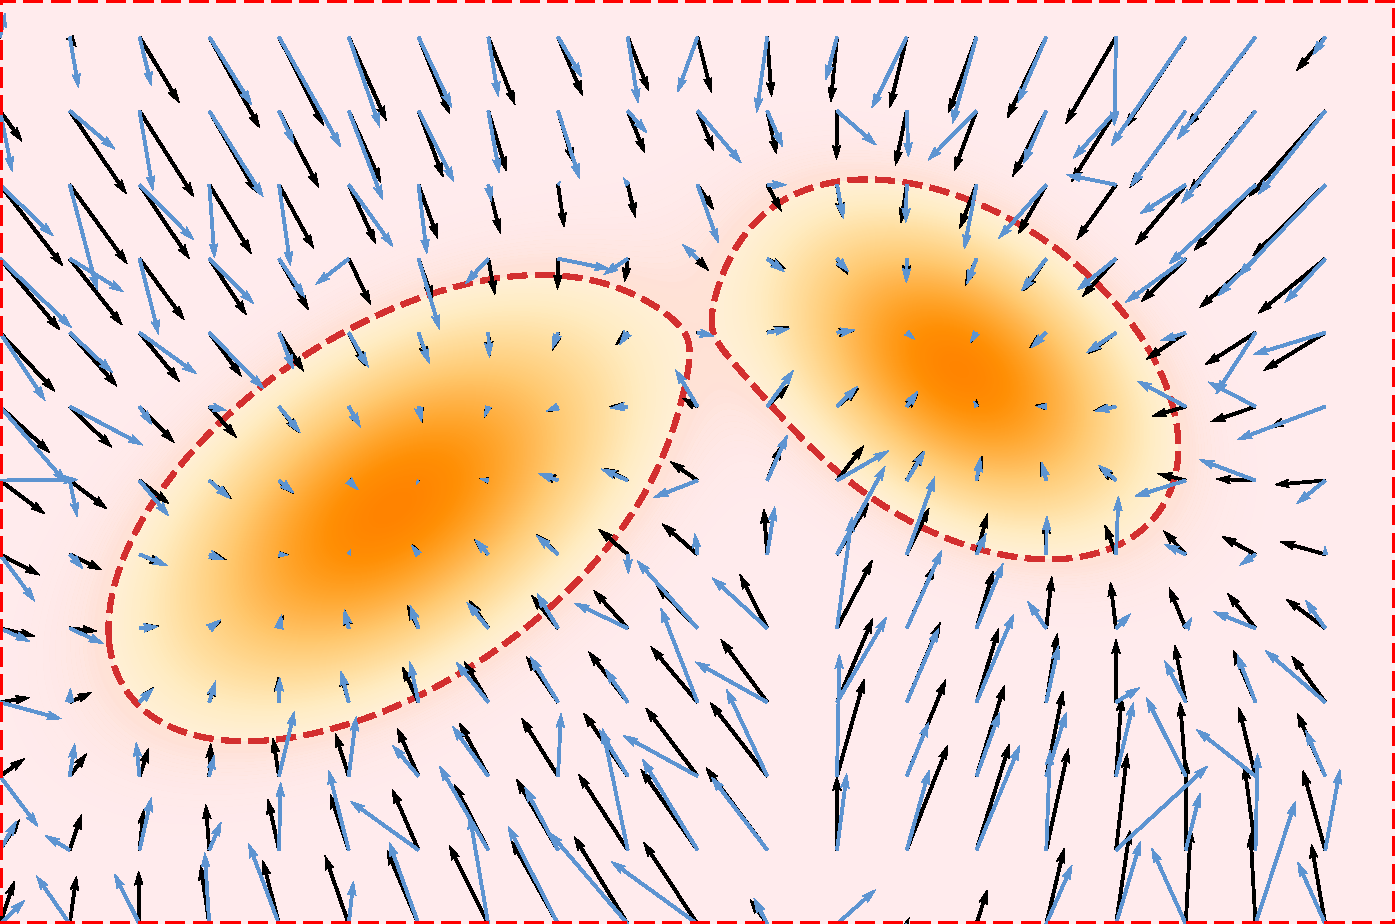
\includegraphics[width=0.85\linewidth]{Images/PartB/score_function_acc.pdf}
    \caption{\textbfs{分数匹配的误差示意（回顾 \Cref{fig:sm-illustration}）。} 红色区域表示低密度区域，由于样本覆盖有限，此处的分数估计可能不准；高密度区域的估计往往更准确。 \figcredit{由作者创建。}}
    \label{fig:sm-acc-illustration}
\end{figure}

为应对这些挑战，\citet{song2019generative} 提出在数据分布的多个噪声水平上注入高斯噪声，并联合训练一个噪声条件分数网络（NCSN），以估计一系列噪声尺度下的分数函数。生成时，朗之万动力学以噪声退火的方式运行：先在高噪声水平上做粗略探索，再逐步过渡到低噪声水平以恢复细节。




\begin{figure}[th]
    \centering
    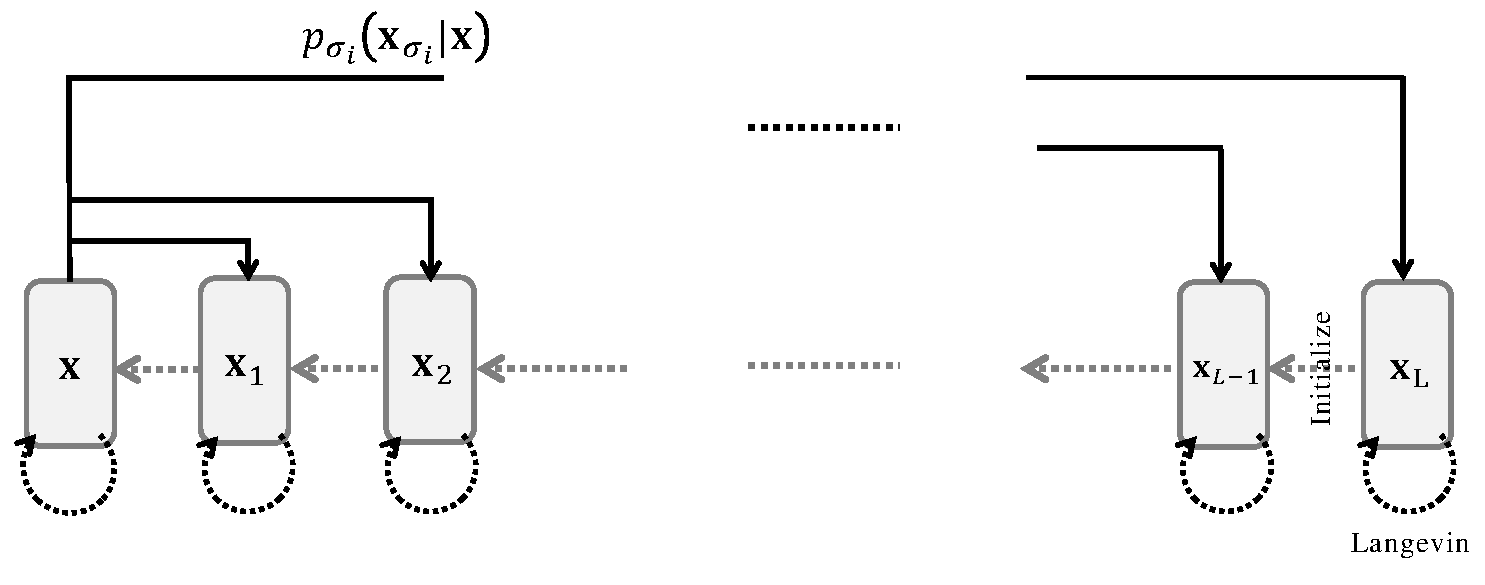
\includegraphics[width=0.95\linewidth]{Images/PartB/ncsn-graph.pdf}
    \caption{\textbfs{NCSN 示意图。} 前向过程用多个水平的加性高斯噪声 $p_{\sigma}(\rvx_{\sigma} | \rvx)$ 扰动数据。生成过程（虚线）在每个噪声水平上做朗之万采样，并用当前水平的结果去初始化下一、更小方差水平上的采样。 \figcredit{由作者创建。}}
    \label{fig:smld-ddpm-graphical-model}
\end{figure}


\subsection{训练}
为克服在单一噪声水平上训练基于分数模型的局限，\citet{song2019generative} 提出在数据分布上加入多个水平的高斯噪声。具体做法是选取一串 $L$ 个噪声水平 $\{\sigma_i\}_{i=1}^L$，满足
\[
0 < \sigma_1 < \sigma_2 < \cdots < \sigma_L,
\]
其中 $\sigma_1$ 足够小，以保留数据的大部分细节；$\sigma_L$ 足够大，能把分布充分平滑，使训练更容易。

每个带噪样本都由干净数据点 $\rvx \sim p_{\text{data}}$ 扰动而成，即 $\rvx_{\sigma} = \rvx + \sigma \bm{\epsilon}$，其中 $ \bm{\epsilon} \sim \mathcal{N}(\bm{0}, \rmI)$。这定义了
\vspace{-0.4cm}
\subparagraph{扰动核：}
\[
p_{\sigma}(\rvx_{\sigma} | \rvx) := \mathcal{N}(\rvx_{\sigma}; \rvx, \sigma^2 \rmI),
\]
由此得到
\vspace{-0.4cm}
\subparagraph{边缘分布：}
\[
p_\sigma(\rvx_{\sigma}) = \int p_{\sigma} (\rvx_{\sigma} | \rvx)    p_{\text{data}}(\rvx) \diff \rvx,
\]
它对每个噪声水平 $\sigma$ 都成立，呈现的是高斯平滑后的数据分布。

\paragraph{NCSN 的训练目标。}\mbox{}\\

目标是训练一个噪声条件分数网络 $\rvs_{\bm{\phi}}(\rvx, \sigma)$，对所有的 $\sigma \in \{\sigma_i\}_{i=1}^L$ 估计分数函数 $\nabla_{\rvx} \log p_\sigma(\rvx)$。做法是在所有噪声水平上最小化 DSM 目标：
\begin{align}\label{eq:nscn}
\mathcal{L}_{\text{NCSN}}(\bm{\phi}) := \sum_{i=1}^{L} \lambda(\sigma_i)   \mathcal{L}_{\text{DSM}}(\bm{\phi}; \sigma_i),
\end{align}
其中
\begin{align*}
\mathcal{L}_{\text{DSM}}(\bm{\phi}; \sigma)
= \frac{1}{2} \mathbb{E}_{\rvx \sim p_{\text{data}}(\rvx),   \tilde{\rvx} \sim p_{\sigma}(\tilde{\rvx} | \rvx)}
\left[ \norm{\rvs_{\bm{\phi}}(\tilde{\rvx}, \sigma) - \left( \frac{\rvx - \tilde{\rvx}}{\sigma^2} \right)}_2^2 \right],
\end{align*}
$\lambda(\sigma_i)>0$ 是各尺度对应的权重函数。最小化该目标得到的分数模型 $\rvs^*(\rvx, \sigma)$ 能恢复每个噪声水平上的真实分数：
\[
\rvs^*(\cdot, \sigma) = \nabla_{\rvx} \log p_\sigma(\cdot),  \quad \text{对所有的 } \sigma \in \{\sigma_i\}_{i=1}^L,
\]
因为它本质上就是 DSM 最小化（见定理~\ref{thm:sm-dsm}）。



\paragraph{与 DDPM 损失的关系。}
设 $\rvx_\sigma=\rvx+\sigma\boldsymbol{\epsilon}$，其中 $\boldsymbol{\epsilon}\sim\mathcal{N}(\mathbf{0},\mathbf{I})$，并以 $p_\sigma$ 记边缘分布。由 Tweedie 公式，
\[
\nabla_{\rvx_\sigma}\log p_\sigma(\rvx_\sigma)
= -\frac{1}{\sigma} \E \left[\boldsymbol{\epsilon} \middle|  \rvx_\sigma\right].
\]
因此 NCSN 的最优解是真实分数 $\rvs^*(\rvx_\sigma,\sigma)=\nabla_{\rvx_\sigma}\log p_\sigma(\rvx_\sigma)$，而 DDPM 损失 \Cref{eq:ddpm-simple-loss} 下的贝叶斯最优噪声预测器是 $\boldsymbol{\epsilon}^*(\rvx_\sigma,\sigma)=\E[\boldsymbol{\epsilon}|\rvx_\sigma]$。两者通过下式完全等价：
\[
\rvs^*(\rvx_\sigma,\sigma) = - \frac{1}{\sigma} \boldsymbol{\epsilon}^*(\rvx_\sigma,\sigma),
\qquad
\boldsymbol{\epsilon}^*(\rvx_\sigma,\sigma) = - \sigma \rvs^*(\rvx_\sigma,\sigma).
\]
在 DDPM 的设定下，第 $i$ 步的带噪样本可以写成
\[
\sigma_i:=\sqrt{1-\bar{\alpha}_i^2},
\qquad
\rvx_i
=
\bar{\alpha}_i\rvx_0+\sigma_i\beps,
\qquad
\beps\sim\mathcal{N}(\bm{0},\rmI).
\]
因此，分数与最优噪声预测携带的是同一份信息：
\[
\rvs^*(\rvx_i,i)
=
-\frac{1}{\sigma_i}
\E\left[\beps|\rvx_i\right].
\]
换言之，在 DDPM 中预测噪声，与在噪声水平 $i$ 上预测分数，只相差一个已知的比例因子 $1/\sigma_i$，两者等价。关于各类参数化之间的这种等价性，我们将在 \Cref{ch:all-equivalent} 中系统比较与总结。



\subsection{采样}


\begin{algorithm}[th]
\caption{\label{alg:smld} 退火 Langevin Dynamics}
\begin{algorithmic}[1]
\Require 训练分数 $\rvs_{\bm{\phi}^\times}(\cdot,\sigma_\ell)$，
步长 $\eta_\ell$ 和 Langevin 迭代预算 $N_\ell$
对于每个噪声级别 $\ell=L,\ldots,1$；初始化分布
$p_{\mathrm{init}}$
\State $\rvx \sim p_{\mathrm{init}}$
\Statex\Comment{从最大噪声水平的非结构化噪声初始化}
\For{$\ell=L,L-1,\ldots,1$}
    \State $\tilde{\rvx}_0 \gets \rvx$
    \Statex\Comment{从上一级的输出初始化此噪声级别}
    \For{$n=0$ \textbf{至} $N_\ell-1$}
        \State $\bm{\epsilon}_n \sim \mathcal{N}(\bm{0},\rmI)$
        \State $\tilde{\rvx}_{n+1}
        \gets
        \tilde{\rvx}_n
        +\eta_\ell
        \rvs_{\bm{\phi}^\times}(\tilde{\rvx}_n,\sigma_\ell)
        +\sqrt{2\eta_\ell}\,\bm{\epsilon}_n$
    \EndFor
    \State $\rvx \gets \tilde{\rvx}_{N_\ell}$
    \Statex\Comment{将最终状态传递到下一个较小的噪声级别（如果有）}
\EndFor
\Ensure $\rvx$
\end{algorithmic}
\end{algorithm}


在多个噪声水平上都训练好分数网络之后，我们手中有
\[
\rvs_{\bm{\phi}^\times}(\cdot, \sigma_1), \quad\rvs_{\bm{\phi}^\times}(\cdot, \sigma_2), \quad \cdots, \quad \rvs_{\bm{\phi}^\times}(\cdot, \sigma_{L-1}), \quad    \rvs_{\bm{\phi}^\times}(\cdot, \sigma_L),
\]
称为\emph{退火朗之万动力学}（annealed Langevin dynamics）~\citep{song2019generative} 的采样过程，在给定了噪声水平 $0<\sigma_1<\cdots<\sigma_L$ 上训练好的分数之后，由高噪声向低噪声逐步推进来生成样本。它先从一个简单的初始化 $\rvx\sim p_{\mathrm{init}}$ 出发，在最大噪声水平 $\sigma_L$ 上做朗之万动力学，用分数 $\rvs_{\bm{\phi}^\times}(\cdot,\sigma_L)$ 把样本推向相应的平滑分布 $p_{\sigma_L}$；再用得到的样本去初始化下一个较小噪声水平上的朗之万动力学。如此反复，样本逐步被细化，直到抵达最小噪声水平 $\sigma_1$。

在每个噪声水平 $\sigma_\ell$ 上，朗之万动力学执行的更新为
\[
\tilde{\rvx}_{n+1}
=
\tilde{\rvx}_n
+
\eta_\ell
\rvs_{\bm{\phi}^\times}(\tilde{\rvx}_n,\sigma_\ell)
+
\sqrt{2\eta_\ell}\,\bm{\epsilon}_n,
\qquad
\bm{\epsilon}_n\sim\mathcal{N}(\bm{0},\rmI),
\]
其初始化 $\tilde{\rvx}_0$ 由上一噪声水平的输出给出。常用做法是让步长随噪声水平缩放：
\[
\eta_\ell
=
\delta\frac{\sigma_\ell^2}{\sigma_1^2},
\qquad
\delta>0.
\]
算法在每个噪声水平上都执行朗之万更新，包括 $\sigma_1$，因此最终的样本是在最小噪声水平上细化之后得到的。\Cref{alg:smld} 概括了这一流程。

初始分布 $p_{\mathrm{init}}$ 只是为马尔可夫链提供一个起点。在最大噪声水平上，朗之万动力学把这个初始分布推向 $p_{\sigma_L}$；随后各个噪声水平接力，把样本逐渐引导到平滑程度越来越低的数据分布上。

\paragraph{NCSN 采样慢。}
NCSN 借助退火 MCMC（通常是朗之万动力学）在一系列噪声尺度 $\{\sigma_i\}_{i=1}^L$ 上生成样本。对每个尺度 $\sigma_i$，它执行 $K$ 次如下形式的迭代更新：“用分数 $\rvs_{\bm{\phi}^\times}(\tilde{\mathbf{x}}_n,\sigma_i)$ 加上一个小的随机扰动来更新 $\tilde{\mathbf{x}}_n$”，而每一次更新都需要通过分数网络做一次前向传播。有两个因素使得 $L \times K$ 必须很大：
\begin{enumerate}
    \item[(i)] \textbfs{局部精度与稳定性：} 学到的分数只在小扰动范围内可靠，因此需要较小的步长，并在每个噪声水平上迭代多次，以避免偏差或不稳定；
    \item[(ii)] \textbfs{高维空间中的混合慢：} 局部 MCMC 移动在探索多模态、高维目标时效率很低，需要大量迭代才能到达数据的典型区域。
\end{enumerate}
由于更新严格串行（每次迭代都依赖上一次），且每次都需一次昂贵的网络求值，总体代价为 $\mathcal{O}(LK)$ 次串行网络前向，采样因而在计算上很慢。











\clearpage
\newpage

\section{总结：NCSN 和 DDPM 的比较}

我们先比较 NCSN 与 DDPM 的图模型（见 \Cref{fig:smld-ddpm-graphical-model}），主要区别与相似之处汇总在 \Cref{tb:comparison-smld-ddpm} 中。


\begin{table}[th]
  \caption{NCSN 与 DDPM 的比较}
  \small
  \centering
  \resizebox{\textwidth}{!}{
  \begin{tabular}{cccc}
     \toprule

         &   \textbfs{NCSN}   & \textbfs{DDPM}  \\
        \midrule
    $\rvx_{i+1}|\rvx_{i}$ & 由 $\rvx_{i+1} =  \rvx_i + \sqrt{\sigma^2_{i+1}-\sigma^2_{i}}\bm{\epsilon}$ 推出   &  \cc{15}定义为 $\rvx_{i+1} = \sqrt{1-\beta_{i}} \rvx_{i} + \sqrt{\beta_{i}}\bm{\epsilon}$  \\
      $\rvx_{i}|\rvx$   & \cc{15}定义为 $\rvx_{i} =  \rvx + \sigma_{i}\bm{\epsilon}$
       &  由 $\rvx_i = \bar{\alpha}_i\rvx + \sqrt{1 - \bar{\alpha}_i^2}\bm{\epsilon}$ 推出 \\
   $p_{\text{prior}}$   & $ \mathcal{N}(\bm{0}, \sigma_L^2\rmI)$    &  $\mathcal{N}(\bm{0}, \rmI)$  \\
   \midrule
        损失
          &
        $\mathbb{E}_{i} \mathbb{E}_{p_{\text{data}}(\rvx)}
        \mathbb{E}_{\bm{\epsilon} \sim \mathcal{N}\left(\mathbf{0}, \rmI\right)}
    \left[ \norm{\rvs_{\bm{\phi}}(\rvx_i, \sigma_i) +   \frac{\bm{\epsilon}}{\sigma_i}}_2^2 \right] $
            &  $      \mathbb{E}_{i}\mathbb{E}_{p_{\text{data}}(\rvx)} \mathbb{E}_{\bm{\epsilon}\sim \mathcal{N}(\bm{0},\rmI)}\left[ \norm{\bm{\epsilon}_{\bm{\phi}}(\rvx_i, i) - \bm{\epsilon}}_2^2 \right]$ \\
    \midrule
     采样   & \begin{tabular}{@{}c@{}} 逐层执行朗之万；\\ 用其输出初始化下一层 \end{tabular}  &  \begin{tabular}{@{}c@{}}遍历马尔可夫链 \\ $p_{\bm{\phi}^\times}(\rvx_{i-1} | \rvx_i)$   \end{tabular} \\
 \bottomrule
  \end{tabular}
  }
  \label{tb:comparison-smld-ddpm}
\end{table}

\paragraph{共同的瓶颈。}
尽管 NCSN 与 DDPM 的表述不同，两者都依赖稠密的时间离散化。这带来一个关键限制：采样往往需要数百乃至数千次迭代，生成因此既慢又费算力。

\begin{question}\label{ques:dm-sampling-slow}
    怎样加速扩散模型的采样？
\end{question}
我们将在后续三章中分别回到这一挑战：\Cref{ch:solvers} 发展更高效的采样器；\Cref{ch:distillation} 把一个需要数百步采样的预训练扩散模型压缩成步数更少的学生生成器；\Cref{ch:fast-scratch} 则研究如何在扩散思想的启发下，直接从零训练出快速的少步生成器。







\newpage

\section{结束语}\label{sec:ch3_cr}



本章从植根于能量模型（EBM）的分数视角出发，勾勒出通往扩散模型的第二条主线。我们首先指出 EBM 的核心难题——难以计算的配分函数——并引入分数函数 $\nabla_{\mathbf{x}}\log{p(\mathbf{x})}$，它是一件能完全绕开该难题的利器。

这一路我们从经典分数匹配走到它更可扩展、更稳健的变体，即去噪分数匹配（DSM）。借助 DSM 我们看到，用噪声扰动数据就能得到易于处理的训练目标，这里又一次利用了条件化技巧，把问题化为简单的回归目标。进一步，我们通过 Tweedie 公式在分数估计与去噪之间建立了深刻的联系：分数所给出的方向，正是从带噪观测估计干净信号所需的方向。

随后，这一原理从单一噪声水平推广到由噪声条件分数网络（NCSN）刻画的\emph{噪声阶梯}：网络学习以多个噪声尺度为条件的单一分数模型，并借助退火朗之万动力学生成样本。下一章将再进一步，通过 Score SDE 框架把这个离散的噪声阶梯过渡到连续的噪声水平。



这种趋同绝非巧合，它暗示着背后有一个更深、更统一的数学结构。而这些离散时间模型的局限，正说明需要一个更一般的框架。下一章我们将迈出这关键一步：
\begin{enumerate}
    \item 我们将转入连续时间视角，说明 DDPM 与 NCSN 都可以被优雅地统一为同一个由随机微分方程（SDE）刻画的强大过程的不同离散化。
    \item 这一 Score SDE 框架将把变分视角与分数视角正式联系起来，并把生成问题改写为求解一个微分方程。
\end{enumerate}

这一统一视角不仅带来理论上的透彻理解，还会解锁一类新的高等数值方法，用以应对采样缓慢这一根本挑战。
